\chapter{Unidad teórica: Clima Espacial Regional}

\section{Introducción}

\subsection{Tormentas geomagnéticas}

Las tormentas geomagnéticas (TG) son fenómenos importantes en el clima espacial debido a su impacto en sistemas de comunicación, navegación y abastecimiento de energía \cite{schrijver2015}. Las TG están estrechamente relacionadas con la actividad solar y , en términos generales, involucran un debilitamiento temporal del campo magnético terrestre (CMT) (Véase Figura \ref{tgm_ex}), así como otros efectos subsecuentes en la atmósfera y subsuelo \cite{gonzalestgm}. 
\vspace{1 em}

Éstas tormentas surgen cuando material (partículas eléctricamente cargadas) proveniente del viento solar penetra dentro del CMT a través del mecanismo de la reconexión magnética entre el CMT y el campo magnético interplanetario (CMI) \cite{l_basic_spaceplasmaphysic, l_russell}. Una vez dentro del sistema CMT, las partículas provenientes de viento solar se integran a las corrientes magnetosféricas lo que conlleva a una intensificación de éstas \cite{l_basic_spaceplasmaphysic}. Una de las corrientes que regularmente es intensificada es la corriente ecuatorial del anillo, intensificación que induce un campo magnético que se opone vectorialmente al CTM. Como consecuencia a esto, se observa una disminución a escala planetaria en la intensidad del CTM, que es especialmente clara la componente horizontal ($H$) en latitudes geomagnéticas medias y bajas.
\vspace{ 1 em}

\section{Respuesta geomagnética}

Las TG son típicamente identificadas usando los índices geomagnéticos, los cuales son herramientas para identificar, clasificar una TG, así como cuantificar su magnitud. Existen varios tipos de índices geomagnéticos, cada uno diseñado para cuantificar aspectos específicos de la respuesta geomagnética. En el caso de las latitudes geomagnéticas medias y bajas, los índices más utilizados son el índice K planetario (${\rm K_P}$) y el índice de tiempo de perturbación por tormenta o \emph{Disturbance Time Storm} (${\rm Dst}$). Éstos índices son especialmente efectivos en regiones donde la perturbación geomagnética puede ser observada en la componente horizontal (H) del CMT. El  \href{https://www.gfz-potsdam.de/en/section/geomagnetism/data-products-services/geomagnetic-kp-index}{índice ${\rm K_P}$} cuantifica la variación, no cíclica, máxima en H observada para intervalos de cada tres horas. Por otro lado, el \href{https://wdc.kugi.kyoto-u.ac.jp/dstae/index.html}{índice ${\rm Dst}$} representa un promedio de perturbación horaria en la componente H de las variaciones no cíclicas alrededor del ecuador geomagnético. Los índices ${\rm K_P}$ y ${\rm Dst}$ cuentan con contrapartes regionales que se calculana partir de datos regionales, en lugar de promedios planetarios \cite{mayaud1980}. 
\vspace{ 1 em}


\begin{figure}[h!]
	\begin{center}
 		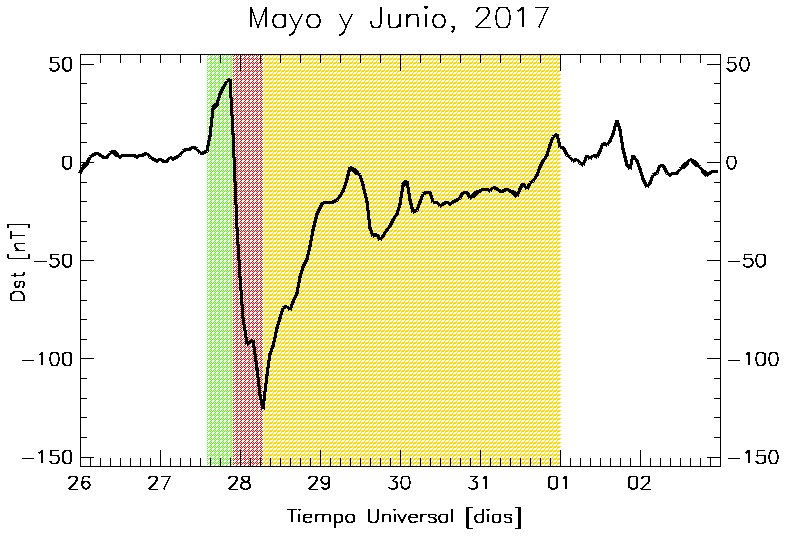
\includegraphics[width = 0.7\textwidth]{Images/dst_ex2017-05-26.png}
 	\end{center}
 	\caption{\label{tgm_ex} Ejemplo de una tormenta geomagnética acontecida a finales de mayo del 2017, cuya evolución en el tiempo es observada a través del índice geomagnético Dst. Con las regiones sombreadas se señalan las diferentes fases de la tormenta. Datos del índice Dst obtenidos de \cite{idx}} 
\end{figure}

La Figura \ref{tgm_ex} muestra un ejemplo de una tormenta geomagnética visto a través del índice Dst. En la figura se aprecian regiones sombreadas que resaltan las tres fases de una TGM: de verde el comienzo súbito, seguido por la fase principal (zona roja) y finalmente la zona amarilla sombrea a la fase de recuperación. La fase principal es un rápido decremento (valores negativos) en la intensidad de la componente horizontal a bajas latitudes del CTM. Esta etapa temporalmente coincide con la reconexión magnética entre el CMI y el CMT. La duración de esta fase principal está determinada por las condiciones del CMI y puede durar desde minutos, hasta horas \cite{l_handbook_geof_sw_Geom_field}. Al terminar la reconexión magnética la taza de inyección de partículas provenientes del VS cesa, iniciado la fase de recuperación (región de color amarillo en la figura). Durante esta fase, en ausencia del flujo de partículas anómalas, la corriente del anillo tiende a perder el exceso de partículas cargadas debido a la recombinación y la dispersión por ángulo de paso. Esto provoca un retorno gradual de la corriente del anillo a su estado pre-tormenta, lo cual provoca un debilitamiento gradual en el campo magnético inducido que se oponía al CMT. Este proceso provoca una recuperación gradual en la magnitud del CMT para eventualmente recuperar su valor pre-tormenta. Esta fase puede durar desde horas hasta varios días, dependiendo de la intensidad de la misma TGM y de las condiciones del CMI.
\vspace{ 1 em}

En ocasiones se puede presentar una fase conocida como \emph{comienzo súbito}, señalada por la región de color verde en la Figura \ref{tgm_ex}. Esta ocurre cuando, al llegar un fenómeno desencadenante (generalmente una EMC), este viene precedido por una onda de choque o región de alta presión. Cuando una onda de choque impacta a la magnetopausa, genera un efecto compresivo sobre toda la magnetosfera terrestre. Esta compresión produce una rápida intensificación del campo magnético a nivel planetario, intensificación que se percibe como un incremento en la intensidad de la componente horizontal del CMT. El comienzo súbito tiene puede durar minutos o pocas horas \cite{l_handbook_geof_sw_Geom_field} y termina al iniciar la fase principal de la tormenta (reconexión magnética).
\vspace{1 em}

\subsection{Índices geomagnéticos Dst $\Delta {\rm H}$ y SYM-H}
El índice Dst es un índice global y es el más ampliamente usado para medir la actividad magnética en latitudes bajas. Se trata de la magnitud normalizada de la componente horizontal del campo Dst (axially symmetric disturbance), como se determina de los datos de 4 observatorios de latitud baja distribuidos longitudinalmente \cite{l_handbook_geof_sw_Geom_field}. Este índice es pensado como una medida de la actividad en la corriente del anillo en tiempos de TG \cite{gombosi_1998}. Su registro es medido cada hora. Los días quietos de cada año son utilizados para establecer un promedio mínimo de la actividad en esta corriente, así como del campo magnético de fondo. Esto se resta de los registros por lo que solo las perturbaciones de esta línea base son registrados. El promedio a nivel mundial es usado a partir de 4 estaciones \cite{hargreaves_1992}. Consecuentemente, con este índice se pueden medir los cambios asociados a la intensificación en la corriente del anillo en tiempos de TG.
\vspace{1 em}

Por otro lado, con el índice $\mathrm{\Delta H}$ se determinan las condiciones del \emph{CTM} en su componente H para una escala regional. Los valores de este índice se derivan entonces, a partir de estaciones magnéticas localizadas dentro del área de estudio de interés \cite{l_handbook_geof_sw_Geom_field}. Como cada estación proporciona valores del \emph{CTM} locales, de cada estación se derivará un índice $\mathrm{\Delta H}$ distinto. Al igual que con el índice Dst, las TG generan valores negativos de campo magnético, por lo que cuanto más intensa sea una tormenta, más negativos serán los valores determinados por este índice.
\vspace{1 em}



%\subsubsection{Índice geomagnético SYM-H}
De forma adicional, a escala planetaria también se utiliza el índice SYM-H. Este índice tiene como propósito el de describir perturbaciones geomagnéticas, siendo a latitudes medias el rango en el que tiene mayor confiabilidad, en términos de perturbaciones simétricas para la componente H del \emph{CTM}. Para fines prácticos, el índice SYM-H es el equivalente del índice que Dst, pero con una cadencia de minutos en lugar de horas. \cite{idx}.\\
\vspace{1 em}

\subsection{Índice geomagnético K}

El índice K indica la intensidad de las variaciones relacionadas con perturbaciones geomagnéticas, incluyendo los efectos de impulso, pero excluyendo efectos de recuperación \cite{BARTELS_kp}. La información del índice es condensada en una escala cuasi-logarítmica, válida para estaciones en latitud geomagnética media, en el rango de los $50^\circ$. Cada estación debe elaborar su propia tabla para asignar valores de K a partir de los límites de saturación que pueden indicarse con el límite inferior para K=9. 
\vspace{1 em}

El índice K planetario (o \emph{Kp}) por otro lado, indica la intensidad de la actividad geomagnética en intervalos de tres horas, siendo un promedio estandarizado de los índices K de 12 observatorios seleccionados. Una estación estándar de esas cuenta con 500 nT como límite inferior de K=9.

\section{Manifestaciones regionales}

Mientras que las TG son fenómenos de escala global, pueden presentarse diferentes variaciones a escala regional de sus efectos. Estas variaciones pueden atribuirse a la heterogeneidad del sistema terrestre, la asimetría de sistemas de corrientes magnetosféricos e ionosféricos, así como a las interacciones entre la magnetosfera y la ionosfera en cada región. Consecuentemente, la latitud geomagnética, el tiempo local y las variaciones estacionales pueden influir en el desarrollo de una TG a nivel regional. No considerar estos factores puede conducir a incertidumbres y malinterpretaciones al intentar comprender los potenciales efectos de las TG\cite{gic_intro, gic, gic_2, gic_brazil}.  
\vspace{1 em}

La latitud geomagnética es un factor que debe tomarse en cuenta en el estudio del clima espacial regional. A mayor altitud, los efectos relacionados con las TG son más intensos. Es por ello que durante mucho tiempo, los estudios enfocados en regiones de latitudes geomagnéticas altas ($\ge 50^{\circ}$), pasando por alto regiones en latitudes medias y bajas.
\vspace{1 em}

Sin embargo, en décadas recientes, ha habido un creciente interés en estudiar los fenómenos asociados al clima espacial en regiones de latitudes medias y bajas. Se puede resaltar estudios de \cite{gic_czech, gic_brazil}, y \cite{gic}, los cuales se enfocan en investigar estos fenómenos en latitudes medias y bajas. En el caso de México, un país situado dentro de los rangos latitudinales ya mencionados, se ha echo un esfuerzo para realizar estudios magnéticos e ionosféricos \cite{MEXART2003, MEXART2005, lenica, MEXART_iono_dist, MEXART_iono_dist2, mario_rodriguez2011, lopez-montes, mario_rodriguez2014, iono-resp2016}. 

\subsection{Influencia de la Ionosfera}
\label{diono}

Se ha identificado el rol potencial de las perturbaciones ionosféricas en la inducción de respuesta geomagnética regional durante periodos de tormenta \cite[see][]{esmeralda, dramaria_1, dramaria7, P-corona1, P-corona2}. Esto es consistente con otros estudios realizados para regiones de latitud media-baja, donde se han descubierto y estudiado dos fuentes principales de variaciones geomagnéticas. Estas son las corrientes ionosféricas de dinamo perturbado o \emph{Ddyn} (por sus siglas en ingles) \cite{blanc_ddyn} y la corriente de perturbación polar número 2 o \emph{DP2} (por sus siglas en ingles) \cite{nishida_68_coherence, nishida_68_fluctuations, nishida_66_knee}.
\vspace{1 em}

Por un lado, \emph{DP2} se relaciona directamente con los campos eléctricos inducidos durante la reconexión magnética. Como se observa en la Figura \ref{fig:dp2_diag}, éstos campos eléctricos son transportados a lo largo de las corrientes de Birkeland \cite{dp2PPEF, dp2_diag}, eventualmente alcanzan la ionosfera en latitudes altas en donde inducen un par de celdas convectivas las cuales se les conoce como de perturbación polar. Las partículas cargadas en la zona entonces comienzan a tener movimiento de deriva por efectos de fuerza centrífuga y de curvatura, lo que resulta en la inducción de un campo eléctrico polarizado \cite{Hepner_a, Hepner_b, Pudovkin, blanc_caudal, Denisenko}. Durante la fase principal de la TG, éstos campos eléctricos, a la par de la corriente \emph{DP2}, pueden extenderse mas allá de las latitudes altas, cubriendo incluso latitudes bajas\cite{nishida_66_knee, nishida_68_coherence, nishida_andobayashi_67}.
\vspace{1 em}

\begin{figure}
	\centering
	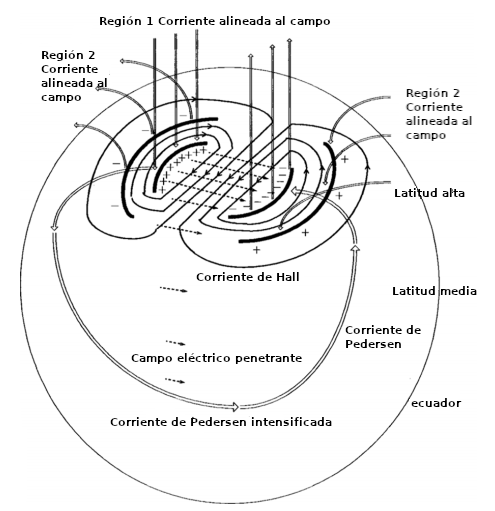
\includegraphics[width=0.5\textwidth]{Images/dp2_edited.png}
	\caption{Representación de la corriente ionosférica $DP2$ teorizada a partir de observaciones \textit{in-situ} realizadas por \cite{nishida_68_fluctuations, nishida_andobayashi_67,nishida_68_coherence}. Las corrientes ionosféricas \emph{DP2}, se componen por un par de corrientes de Hall en latitudes altas y una corriente de Pedersen que fluye en la ionosfera ecuatorial. Figura adaptada de \cite{dp2_diag}.}
	\label{fig:dp2_diag}
\end{figure}


Por otro lado, las \emph{Ddyn} representan amplificaciones de la termósfera polar debido a la precipitación de partículas energéticas durante la fase principal. En la Figura \ref{fig:ddyn_diag}, se observa que el calentamiento de Joule resultante provoca que la termosfera se expanda y tenga  flujos de circulación de viento neutro y partículas cargadas con dirección hacia el ecuador. La fuerza de coriolis induce un cambio de dirección hacia el oeste de estos flujos en latitudes bajas y medias \cite{blanc_ddyn, ddyn2005, angeoddyn}. Como consecuencia, se inducen corrientes de Pedersen y, debido a la acumulación de cargas a lo largo del ecuador magnético en el lado día se terminan generando  campos eléctricos con dirección polar y que se oponen a las primeras corrientes de Pedersen. Finalmente aparecen corrientes de Hall con dirección este, en latitudes medias ($\sim 45^\circ$), las cuales son interrumpidas en los  terminadores\cite{blanc_ddyn}. Esta secuencia de eventos resulta en corrientes divergiendo y cerrándose en latitudes adyacentes, formando un par de corrientes con forma de vórtice, conocidas como dinamo perturbado.
\vspace{1 em}

\begin{figure}
	\centering
	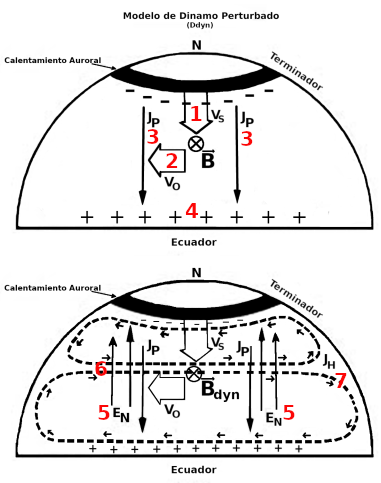
\includegraphics[width=0.5\textwidth]{Images/ddyn_diagedited.png}
	\caption{Representación gráfica del modelo del dínamo ionosférico perturbado ($ddyn$) teorizado y predicho por M. Blanch en 1980. Figura adaptada de \cite{diagrama_ddyn}.}
	\label{fig:ddyn_diag}
\end{figure}

Considerando que \emph{Ddyn} y \emph{DP2} poseen el potencial de influir en la respuesta geomagnética en latitudes medias y bajas, lleva a la pregunta si éstos son los mecanismos responsables de las variaciones locales del CMT encima de México. Previamente, \cite{tesis_yo}, estudió los efectos de estas dos corrientes en los registros magnéticos asociados con la presencia de las corrientes ionosféricas $Ddyn$ y $DP2$. En este estudio se encontró que, en general la presencia de $Ddyn$ y $DP2$ sí afectaban el campo magnético local, ocasionando variaciones de naturaleza cuasi-periódica en el mismo. Sin embargo, el número de eventos analizados fue reducido debido a los parámetros considerados para la selección de eventos, así como la disponibilidad y calidad de los datos de campo magnético locales. Lo anterior llevó también a determinadas limitaciones tanto en los datos como en el procedimiento y en el análisis de los resultados. Por ello, se requiere incrementar el estudio precedente a través del análisis de una base de datos mayor. De igual forma, se puede realizar un fortalecimiento de los resultados a través de implementar herramientas de análisis adicionales y mejorar las ya implementadas.







